\documentclass{standalone}
\usepackage{tikz,amsmath,tkz-euclide}
\begin{document}
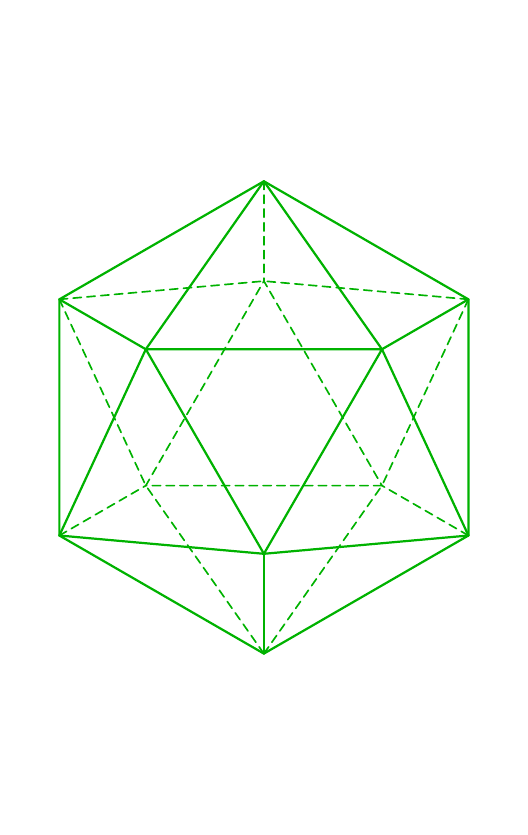
\begin{tikzpicture}[>=latex, scale=1.5]
  \useasboundingbox(-2.0,-3.3)rectangle(2.0,3.3);
  \foreach \x[count=\i] in {30,90,...,330}
  {
    \tkzDefPoint(\x:2){A\i}
  }
  \foreach \x[count=\i] in {30,150,270}
  {
    \tkzDefPoint(\x:1.1547){B\i}
    \tkzDefPoint(-\x:1.1547){C\i}
  }
  \tkzDrawPolygon[thick,green!70!black](A1,A2,A3,A4,A5,A6)
  \tkzDrawPolygon[thick,green!70!black](B1,B2,B3)
  \tkzDrawPolygon[semithick,densely dashed,green!70!black](C1,C2,C3)
  \tkzDrawSegments[thick,green!70!black](A1,B1 A2,B1 A2,B2 A3,B2 A4,B2 A4,B3 A5,B3 A6,B3 A6,B1)
  \tkzDrawSegments[semithick,densely dashed,green!70!black](A1,C1 A2,C3 A3,C2 A3,C3 A4,C2 A5,C2 A5,C1 A6,C1 A1,C3)
\end{tikzpicture}
\end{document}